\documentclass[10pt, a4paper, openany]{book}
\usepackage[italian]{babel}
\usepackage{listings}
\usepackage{graphicx}
\usepackage{fancyvrb}
\usepackage{hyperref}
\usepackage{amsmath}
\usepackage{floatflt,epsfig}
\pagenumbering{arabic}

\graphicspath{ {./images/} }
\renewcommand{\labelenumii}{\arabic{enumi}.\arabic{enumii}}

\begin{document}
\title{RSO - Reti e Sistemi Operativi}
\author{Sara Angeretti}
\date{Gennaio 2023}

\maketitle
\tableofcontents

%Fine indice - Inizio Appunti

\chapter{Introduzione alle reti}
Capitolo 1 (Kurose-Ross 7a edizione).

\noindent Paragrafi: 1.1 - 1.5 (escluso 1.3.2, "circuit switching")

\section{Cos'è una rete}
\subsection{Introduzione ad una rete}
Quando parliamo di Internet sappiamo che parliamo di una \textbf{collaborazione}, una \textbf{cooperazione} fra più server e/o più utenti, organizzati tramite una divisione di ruoli. Questa è possibile solo in caso di \textbf{compatibilità} fra le \textit{tecnologie} e fra gli \textit{standard} scelti.

\vspace{0.5cm}
\noindent \textbf{Alcune terminologie utili}.
\begin{itemize}
    \item Parliamo di \textbf{end system} o \textbf{terminale} per indicare il punto che fa da \textit{capo} alla comunicazione (dove comincia o dove finisce). Sono tutti gli apparati che noi conosciamo visivamente come computer di utenti o server o torri radio\dots
    
    \noindent Non sono da confondere con i \textbf{router} o gli \textbf{switch} (distinguiamo in base a tecnologie fisiche e softwares usati su di essi), che sono \textit{intermediari, nodi} che fanno da tramite alla comunicazione. Un'altra distinzione utile fra switches e routers è la seguente: nella rete, gli \textbf{switches} si trovano dentro la parte di rete più "privata" (domestica ma non solo), mentre i \textbf{routers} si trovano all'esterno di questa parte, nella sezione di rete più pubblica.
    \noindent Questi non sono \textbf{end system}, ma fanno parte della sezione \textbf{core}, che indica la parte più interna e "invisibile" (all'utente che usa un host) della rete.
    \item Parliamo di \textbf{network apps} (\textbf{applicazioni di rete}) per indicare cosa fanno per noi nella comunicazione determinati pezzi di software.
    \item Parliamo di \textbf{bandwidth} (\textbf{larghezza di banda}) per quantificare con un \textbf{numero} (la \textbf{bandwidth} è un \textit{numero}) un certo livello di prestazione della rete che vogliamo valutare. Serve per capire il punto in cui un parametro va bene o va male e perché.
\end{itemize}

\vspace{0.5cm}
\noindent Più nel dettaglio (organizzazione della struttura di una rete come schematizzato nell'immagine). Zone diverse avranno esigenze diverse e quindi soluzioni e strutture diverse.
\begin{center}
    % 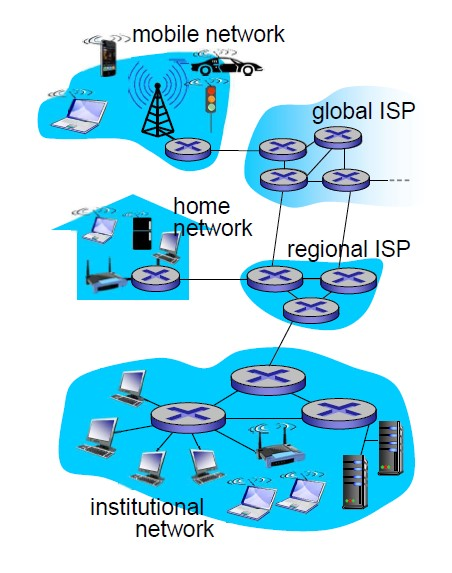
\includegraphics[width=40mm,scale=0.5]{cap1 - Introduzione alle reti - 1.jpg}
    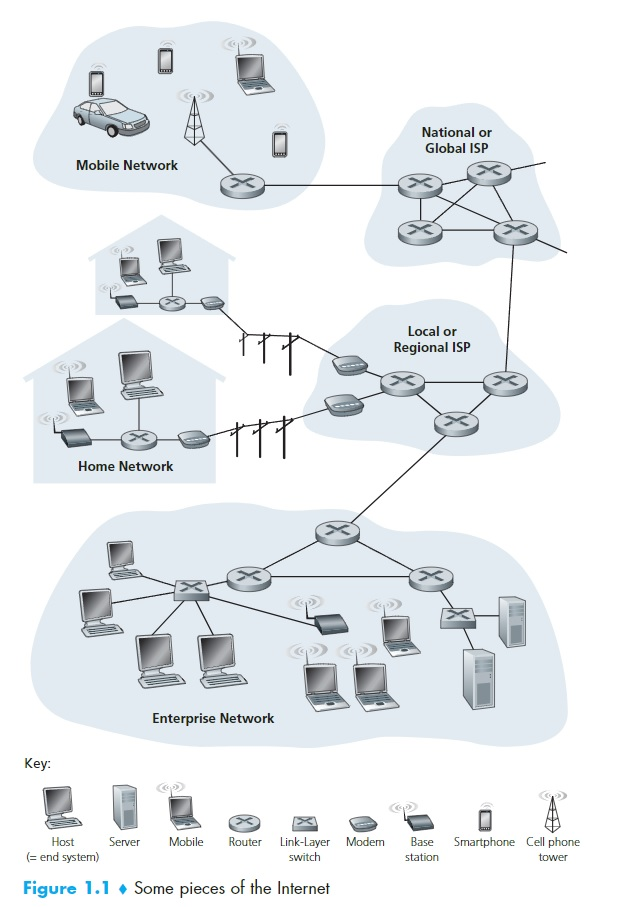
\includegraphics[width=70mm,scale=0.5]{cap1 - Introduzione alle reti - 0.jpg}    
\end{center}
\noindent Nella foto per esempio possiamo vedere in \textit{alto} il lato cliente e in \textit{basso} il lato fornitore.

\vspace{0.5cm}
\noindent \textbf{Altra terminologia}.
\begin{itemize}
    \item Le \textbf{network edges} sono le parti terminali (\textbf{hosts}, che si dividono in \textit{clients} e in \textit{servers}, questi ultimi possono essere raggruppati in \textit{data centers}).
    \item Il \textbf{network core} è tutto ciò che sta "dietro le quinte". Verranno utilizzate tecnologie diverse da quelle delle \textbf{network edges}. Sono gli \textbf{switch} e i \textbf{router}.
    \item Da "tessuto connettivo" delle due aree sopracitate fungono \textbf{access network} e \textbf{physical media}. Sono composti da tutto ciò che mi serve per andare dalla parte \textit{edge} alla parte \textit{core}, quindi punti di \textit{connessione} e \textit{tratti} o \textit{cammini} che possono essere composti da cavi fisici o connessioni senza fili.

    \noindent Esempio: per andare dal mio computer di casa (un \textit{client edge}) al modem del fornitore (lo possiamo vedere come uno \textit{switch}) c'è un cavo, il mio \textit{cammino fisico}.
\end{itemize}

\subsection{Access Network - collegamento}
\noindent Una distinzione che è possibile fare per il concetto di "funzione di \textit{collegamento fisico}" è quella delle diverse implementazioni che questa funzione ha a seconda dell'ambito in cui si trova.
\begin{center}
    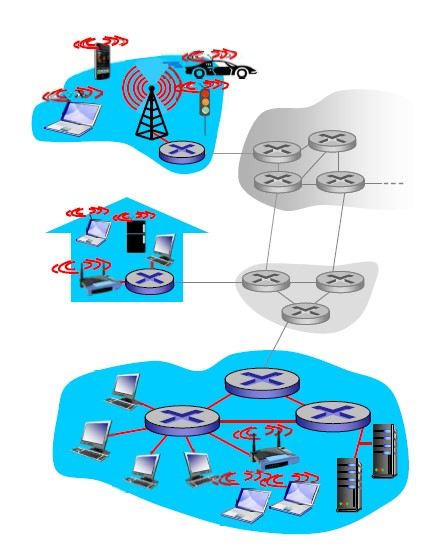
\includegraphics[width=40mm,scale=0.5]{cap1 - Introduzione alle reti - 2.jpg}
\end{center}
\noindent Per esempio, sarà molto diverso fra:
\begin{itemize}
    \item Residential access nets (rete privata).
    \item Institutional access networks (school, company, quindi reti pubbliche).
    \item Mobile access networks (reti mobili).
\end{itemize}
\noindent Per riuscire a fare questa distinzione, bisognerà tenere a mente:
\begin{itemize}
    \item Bandwidth (bits per second).
    \item Shared or dedicated network?
\end{itemize}

\section{Alcuni tipi di reti}
\subsection{Residential access nets - reti private}
% 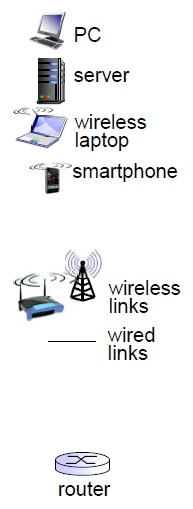
\includegraphics[width=0.2\textwidth]{cap1 - Introduzione alle reti - 3.jpg}
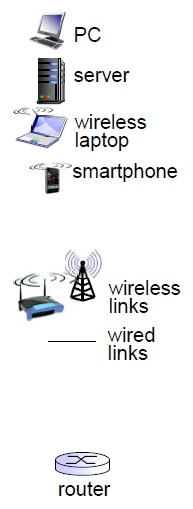
\includegraphics[width=25mm]{cap1 - Introduzione alle reti - 3.jpg}

\noindent Al centro di questa immagine abbiamo un altro esempio di \textbf{router}, fin qui definito uno \textit{strumento tecnologico intermediario} (quindi \textit{core}) nelle reti pubbliche. Ovviamente non c'è mai un solo pc (una \textit{edge}) per un solo fornitore: abbiamo un punto intermedio (\textit{switch} o \textit{WiFi}) che raccoglie le informazioni/connessioni da più pc e le porta al fornitore telefonico (esterno al grafico).

\subsection{Enterprise access nets - Ethernet}
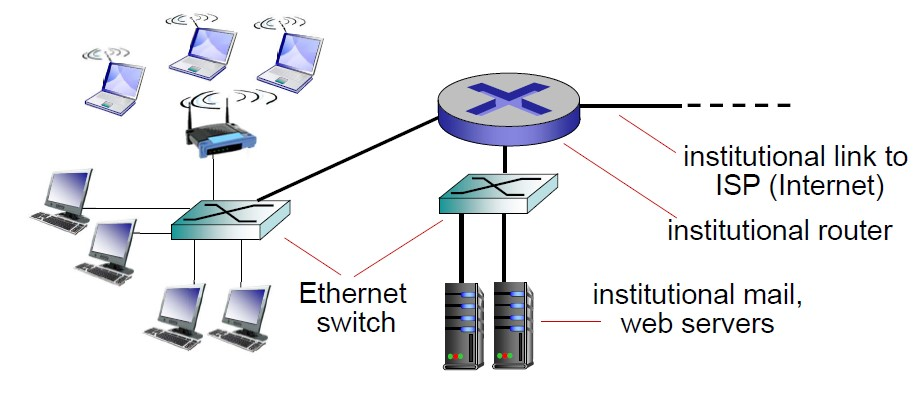
\includegraphics[width=75mm]{cap1 - Introduzione alle reti - 4.jpg}

\noindent Prima tecnologia degna di presentazione. Storicamente una delle più importanti tecnologie di rete, semplice ma interessante da vedere.

\noindent Nel tempo è stata arricchita nelle prestazioni (aumento della larghezza di banda: 10Mbps, 100Mbps, 1Gbps, 10Gbps...), questa sua capacità di raggiungere prestazioni via via più elevate l'ha resa adatta all'uso anche in ambienti aziendali (non solo domestici).

\noindent Ethernet è tipicamente su cavo, sfrutta diversi \textit{ethernet-switch} (a livello datalink, cioè switch, diremo qualcosa di più preciso). Vedremo un capitolo dedicato, che inquadra due livelli: quello \textit{fisico} (che tipo di cavo) e quello \textit{datalink} (come identifico chi è collegato grazie al mio cavo?).

\subsection{Wireless access nets - WiFi}

\noindent Se Ethernet era un esempio di connessione con il cavo, sappiamo che ci sono anche connessioni senza cavo.

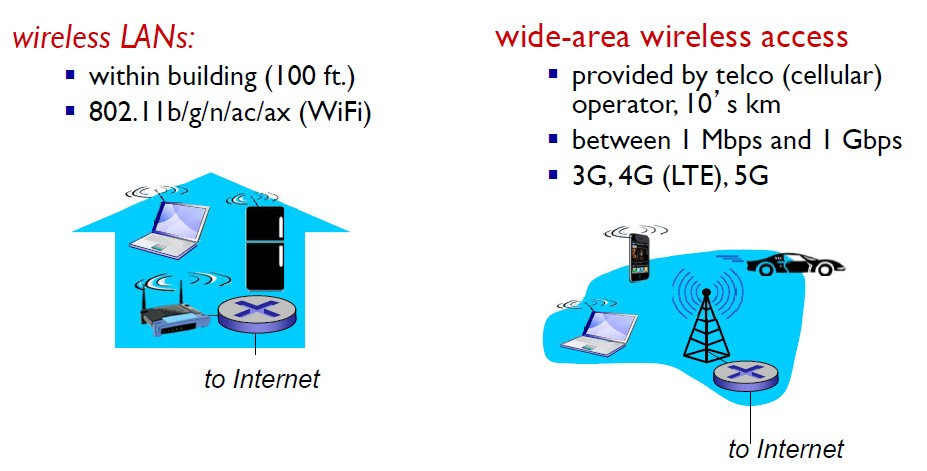
\includegraphics[width=85mm]{cap1 - Introduzione alle reti - 5.jpg}

\noindent Nell'immagine abbiamo l'esempio di \textbf{WiFi} a \textit{sinistra} (tipicamente privata) e di \textbf{4G} a \textit{destra} (tipicamente risorsa delle aziende). Sono entrambi sistemi ad onde radio che collegano gli end-system alla base del fornitore anche nota come "access point (punto di accesso)" tramite una connessione che non prevede cavi.

\section{Frammentazione della comunicazione}

\subsection{Cosa fa l'host - pacchetti di dati}

\noindent Concetto oggi magari banale, ma non tempo fa. In origine la rete dedicava un canale costantemente e in esclusiva a mittente-destinatario, l'intero tempo di uso della rete era loro e esclusivo. Il che vuol dire che finché non finivano di inviare le informazioni, la rete non si liberava. La rivoluzione di 30 e più anni fa è che ora posso andare a \textit{sezionare} o \textit{frammentare} la comunicazione in \textbf{pacchetti} di alcuni bit di lunghezza (circa 1Kb, 8000 bits, è più o meno una misura standard).

\begin{center}
    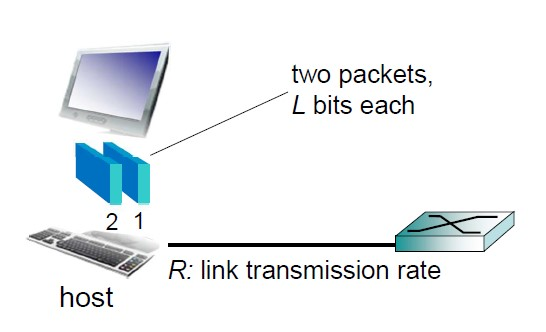
\includegraphics[width=45mm]{cap1 - Introduzione alle reti - 6.jpg}
\end{center}

\noindent Ma di cosa si occupa l'host (\textbf{network edges} o \textit{parti terminali} di una rete) di una rete?
\begin{itemize}
    \item Accetta il messaggio dell'applicazione.
    \item Rompe l'informazione in blocchi più piccoli, noti come pacchetti, di lunghezza \textit{L} bit.
    \item Trasmette il pacchetto nella rete alla velocità di trasmissione \textit{R}, espressa in bit per secondo.
    
    La \textit{velocità di trasmissione del collegamento} è nota anche come \textit{capacità del collegamento} o come \textit{larghezza di banda del collegamento} (\textit{bandwidth}). Soprattutto a livello fisico, si incrocia con il valore della lunghezza del pacchetto.
\end{itemize}

\noindent Vediamo qui la prima \textit{formula}, la prima \textit{quantificazione numerica} di quanto una rete impiega per trasmettere un determinato pacchetto.

\begin{center}
    $delay=\frac{L (bits)}{R (bits/sec)}$
\end{center}

\noindent Il tempo necessario al trasferimento di un pacchetto di \textit{L} bit di lunghezza sulla connessione è il ritardo (\textit{delay}) di trasmissione del pacchetto in questione.

\vspace{0.5cm}

\noindent Ma come colleghiamo i due concetti? Come arriviamo a parlare di \textit{delay} partendo dal tempo di trasmissione di un pacchetto?

\noindent Tanto per cominciare dobbiamo avere ben chiaro il concetto di \textit{tempo di trasmissione} (\textbf{tTX}). Facciamo l'esempio seguente: abbiamo un pacchetto di dati di $L =$ 1000 bit su una rete di $R =$ 1000 bps. Quanto tempo ci vorrà per trasmettere quel pacchetto su quella rete? Ovviamente $tTX = 1 sec$.

\noindent Tutto questo però sulla carta.

\noindent In realtà il vero tempo di trasmissione di un pacchetto è visto più come un \textbf{ritardo} (\textit{delay}): mettiamo di avere l'\textit{istante in cui il \textbf{mittente inizia}}, l'\textit{istante in cui il \textbf{destinatario finisce}} e la distanza tra questi due momenti. Il tempo quindi tra cui il mittente inizia a trasmettere e il momento in cui il destinatario \textit{realmente} ha ricevuto il pacchetto completo, è visto come un \textit{delay}, un "ritardo" fra la disponibilità del dato in trasmissione e disponibilità in ricezione.
% \begin{center}
%     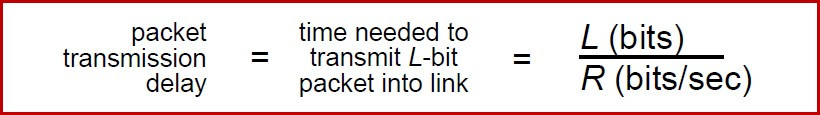
\includegraphics[width=65mm]{cap1 - Introduzione alle reti - 7.jpg}
% \end{center}

\section{Rete e instradamento}

\subsection{Parte core della rete}

\noindent Ovviamente ogni azienda che gestisce l'infrastruttura di comunicazione può usare la sua comunicazione. 

\noindent Quello che importa è che la rete, nell'immagine rappresentato come insieme di tanti punti di transito, è una maglia di router interconnessi.
\begin{center}
    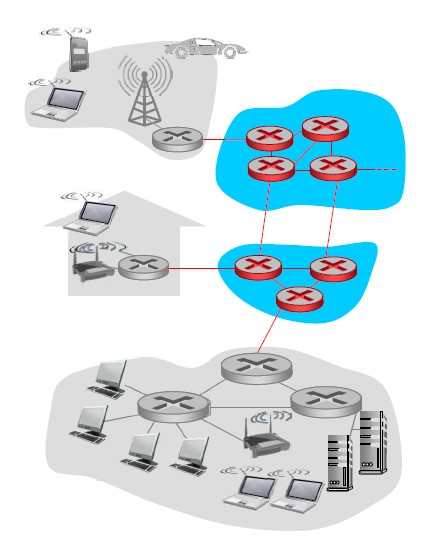
\includegraphics[width=40mm]{cap1 - Introduzione alle reti - 8.jpg}
\end{center}
\noindent Commutazione di pacchetto: gli host frammentano il livello di applicazione messaggi in pacchetti.

\noindent I pacchetti vengono inoltrati da un router al successivo, attraverso collegamenti sul percorso dalla fonte alla destinazione.

\noindent Ogni pacchetto viene trasmesso alla piena capacità della rete.

\subsection{Store and forward.}

\noindent Come precedentemente illustrato, ci vogliono $\frac{L}{R}$ secondi per trasmettere un pacchetto lungo $L$ bit su una connessione ad una velocità (della rete) di  $R$ bps.
\begin{center}
    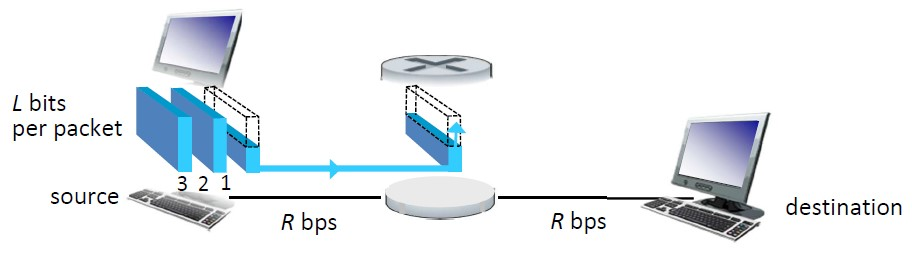
\includegraphics[width=95mm]{cap1 - Introduzione alle reti - 9.jpg}
\end{center}
\noindent Il meccanismo di trasmissione \textit{\textbf{store-and-forward}}, che avviene tra \textit{source} e \textit{destination} tramite un punto intermedio (che prima non consideravo in quanto appartenente alla parte \textit{core}), prevede che la trasmissione dell'\textbf{intero pacchetto} non avvenga "bit a bit" ma solamente una volta che l'\textbf{intero pacchetto} è stato inoltrato e memorizzato, prima di essere nuovamente inviato. Ovviamente:
\begin{itemize}
    \item non stiamo parlando a livello di cavo fisico, dove ovviamente ci sarà una trasmissione "bit a bit" che ci permette quindi di avere una velocità $R$ di trasmissione;
    \item il \textit{nodo intermedio} deve avere uno spazio di deposito del dato per poterlo memorizzare per intero, solo quando sarà lì tutto potrà uscire dal nodo intermedio e quindi inoltrato.
    \item è chiaro che i tempi si allungano, in quanto dovendo ricevere tutto il pacchetto nel nodo intermedio prima di poterlo inoltrare il tempo si raddoppia (e di conseguenza si raddoppia anche il \textit{delay}).
\end{itemize}
\noindent Perciò l'approccio \textit{store-and-forward} ci peggiora la vita per quanto riguarda i tempi, infatti dover aspettare che tutto il pacchetto arrivi nel nodo intermedio fa aspettare di più il destinatario. Vedremo però che migliora l'organizzazione del fluire dei dati. Aiuta a comprendere questo concetto immaginare (tranne che a livello fisico) il pacchetto come un blocco rigido, ogni spostamento avviene per l'intero blocco.

\noindent In conclusione, il tempo di trasmissione da capo a capo (\textit{end-to-end delay}) $= 2\frac{L}{R}$.

\subsection{Packet switching: queueing delay, loss.}

\noindent Vediamo una situazione un po' più concreta (reale) che ci mostra il vantaggio di avere la trasmissione a pacchetto e del condividere tratti di archi di comunicazione fra più computer. Questo vantaggio ha anche degli eventuali problemi che ora vedremo: cioè se più dispositivi condividono uno stesso canale di comunicazione, bisogna fare attenzione che non interferiscano "pestandosi i piedi" a vicenda! Questo perché ovviamente nello stesso canale fisico non possono passare due bit nello stesso istante. 
\begin{center}
    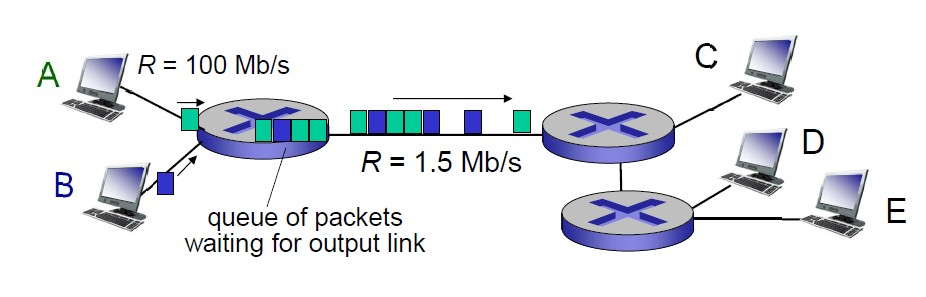
\includegraphics[width=95mm]{cap1 - Introduzione alle reti - 10.jpg}
\end{center}
\noindent Per quanto detto anche riguardo l'approccio \textit{store and forward}, possiamo quindi affermare che sul canale \textbf{condiviso} non avvenga un'alternanza di \textit{bit} ma di \textit{pacchetti}. Ricordando che siamo ancora in modalità \textit{store and forward}, notiamo che nel primo noto intermedio (condiviso da più utenti) c'è un accumulo, un salvataggio dei pacchetti di dati per intero provenienti dai due computer sulla sinistra. Perciò può capitare che si accumulino anche pacchetti di dati molto vecchi e particolarmente lenti ad essere trasmessi (velocità della coda in uscita lenta). Come detto prima il nodo intermedio avrà bisogno di una coda, uno spazio di deposito dei vari pacchetti, che potrebbe tuttavia non essere capiente a sufficienza. Questa cosa può essere vista nell'esempio rappresentato nell'immagine delle due \textbf{velocità in entrata e in uscita} del nodo intermedio.

\noindent Es. tipico: casello autostradale.

\noindent N.B.: i pacchetti, provenienti dai due computer sulla sinistra nell'esempio rappresentato, sul canale condiviso non possono essere trasmessi \textbf{contemporaneamente} ("sul canale fisico non possono passare due bit contemporaneamente"), ma devono essere \textbf{alternati}. È per questo che la coda di immagazzinamento (storing) del nodo intermedio rischia di saturarsi molto velocemente.

\vspace{0.5cm}

\noindent Parliamo di \textbf{accodamento} e \textbf{perdita} (\textbf{queuing and loss}) a livello di nodo intermedio nel caso in cui le velocità di \textbf{entrata} superino per un certo periodo di tempo la velocità di \textbf{uscita} dal nodo. Una volta che il nodo intermedio ha accumulato pacchetti fino a riempire la sua \textbf{limitata} capacità fisica di memoria (\textit{buffer}), se i due computer provano ancora a inviare pacchetti, sorge un problema. La possibile soluzione varia a seconda delle tecnologie:
\begin{itemize}
    \item i pacchetti possono essere persi (dropped, lost), il nodo cioè "butta via" \textit{silenziosamente} i pacchetti;
    \item il nodo \textit{segnala} al trasmittente (i due computer sulla sinistra) di non avere spazio, il trasmittente aspetta accodando i pacchetti che vuole trasmettere.
\end{itemize}

\noindent Tra l'opzione di \underline{mandare indietro il segnale di memoria piena} e invece l'opzione di \underline{buttar via silenziosamente il pacchetto}, \textbf{Internet} sceglie la via più semplice (cioè la seconda). Sarà quindi compito del \textbf{mittente} (i due computer) accorgersi che il pacchetto inviato non è stato ricevuto dal nodo intermedio. TCP è un esempio di standard che si occupa di questo.

\noindent Obiettivo finale: nodi diversi si occupano di problemi diversi, i nodi intermedi nella loro versione semplice si occupano solo di prendere ed inoltrare.

\vspace{0.5cm}

\noindent \underline{\textit{Nuovo problema}}: nel caso di più uscite da un singolo nodo intermedio, come facciamo a capire dove deve andare il pacchetto da trasmettere? Ovviamente dipende dal \textbf{destinatario}. In base alla destinazione ho una scelta di percorso. Ma non solo: dipende anche dalla \textbf{situazione} (per esempio un nodo intermedio non funziona più). È una questione abbastanza estesa, ci dedicheremo un capitolo intero nella sezione del \textit{livello di rete (network)}. Il succo è che la scelta di quale percorso seguire in base alla situazione in cui mi trovo è dettata da specifici algoritmi. Ma Internet fa del suo meglio (\textit{best effort}).

\subsection{Routing and forwarding.}

\noindent Introduciamo i termini \textbf{instradamento} (\textbf{routing}) e \textbf{inoltro} (\textbf{forwarding}).

\begin{itemize}
    \item il \textbf{routing} è una scelta del percorso che dipende dall'\textit{algoritmo di instradamento} o \textit{di routing};
    \item il \textbf{forwarding} è semplicemente un nodo passa l'informazione ad un altro nodo.
\end{itemize}

\subsection{Altro sui tempi di trasmissione, \textit{delay} e \textit{loss}.}

\begin{center}
    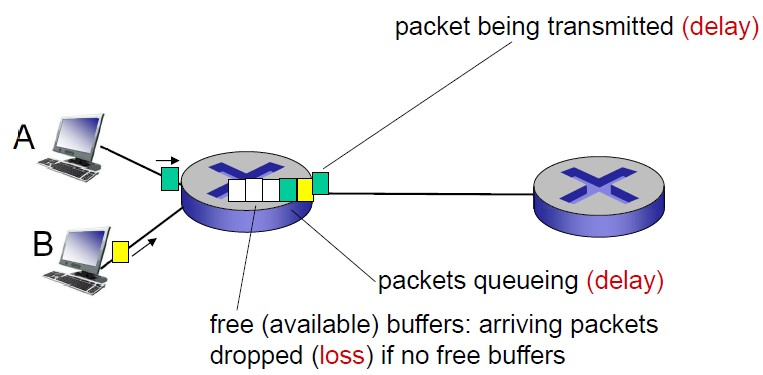
\includegraphics[width=75mm]{cap1 - Introduzione alle reti - 21.jpg}
\end{center}
\noindent Come abbiamo già illustrato, i pacchetti provenienti dai computer \textit{A} e \textit{B} vengono trasmessi con due velocità (presumibilmente) diverse al nodo intermedio (di sinistra): qui vengono accodati per essere poi trasferiti al nodo successivo (qua a destra) tramite un cavo.

\noindent Questo cavo (fisico) abbiamo detto ha una velocità sua di trasferimento. Per spostarsi tra i due nodi intermedi, i pacchetti ci mettono un tempo fisico pari a $\frac{L}{R}$ che è il minimo tempo strettamente necessario per attraversare il cavo. Questo tempo, sommato al tempo che i pacchetti passano in coda nel primo nodo intermedio, mi dà il \textit{ritardo} o \textit{delay} dei pacchetti (dato sia dal \textit{ritardo di trasferimento} dei pacchetti da nodo intermedio all'altro e dal \textit{ritardo di accodamento} su un nodo).

\noindent Questo secondo tempo (di accodamento) non lo conosciamo ed è difficile da determinare, in quanto è \textit{transitorio}, cioè dipende dalla situazione in cui ci troviamo e potrebbe variare in modo abbastanza \textit{imprevedibile}.

\noindent Un'altra cosa che potrebbe variare in modo abbastanza imprevedibile è ciò che abbiamo chiamato \textit{loss}, ovvero l'eventuale perdita di dati.

\noindent Come abbiamo precedentemente già detto, la perdita (\textit{loss}) dei dati avviene perché la coda (\textit{buffer}) del nodo intermedio immediatamente precedente a dove ci troviamo ha dimensione \textit{finita} ma i pacchetti di informazione continuano ad arrivare anche quando è completamente piena. L'informazione persa può essere trasmessa di nuovo dal mittente, dal nodo intermedio oppure persa per sempre.

\subsection{Quattro sorgenti di \textit{delay} nella trasmissione di pacchetti.}

\begin{center}
    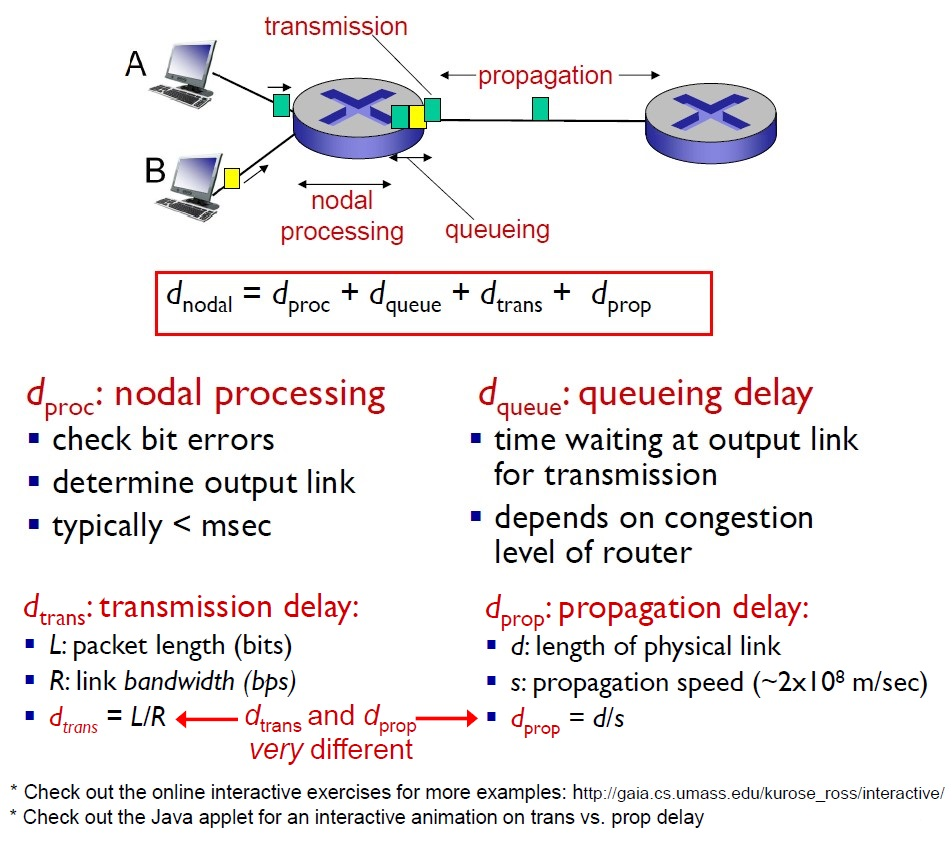
\includegraphics[width=80mm]{cap1 - Introduzione alle reti - 22.jpg}
\end{center}
\noindent L'immagine prova a modellare quanto detto finora. 

\noindent N.B.: l'immagine illustra solo il \textit{delay}, non considera l'eventuale \textit{loss}.

\vspace{0.5cm}

\noindent Perciò il tempo reale di attraversamento (salto) di un nodo è:
\begin{center}
    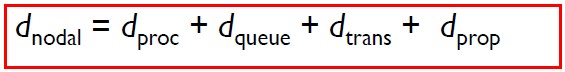
\includegraphics[width=60mm]{cap1 - Introduzione alle reti - 23.jpg}
\end{center}

\vspace{0.5cm}
\noindent Un esempio pratico per capire quanto importante sia questo concetto della propagazione fisica è la vecchia Ethernet di una volta.

\noindent Immaginiamo di avere un cavo coassiale con tre stazioni. A livello fisico, è \textbf{condiviso} (aka tutti vedono tutti).
\begin{center}
    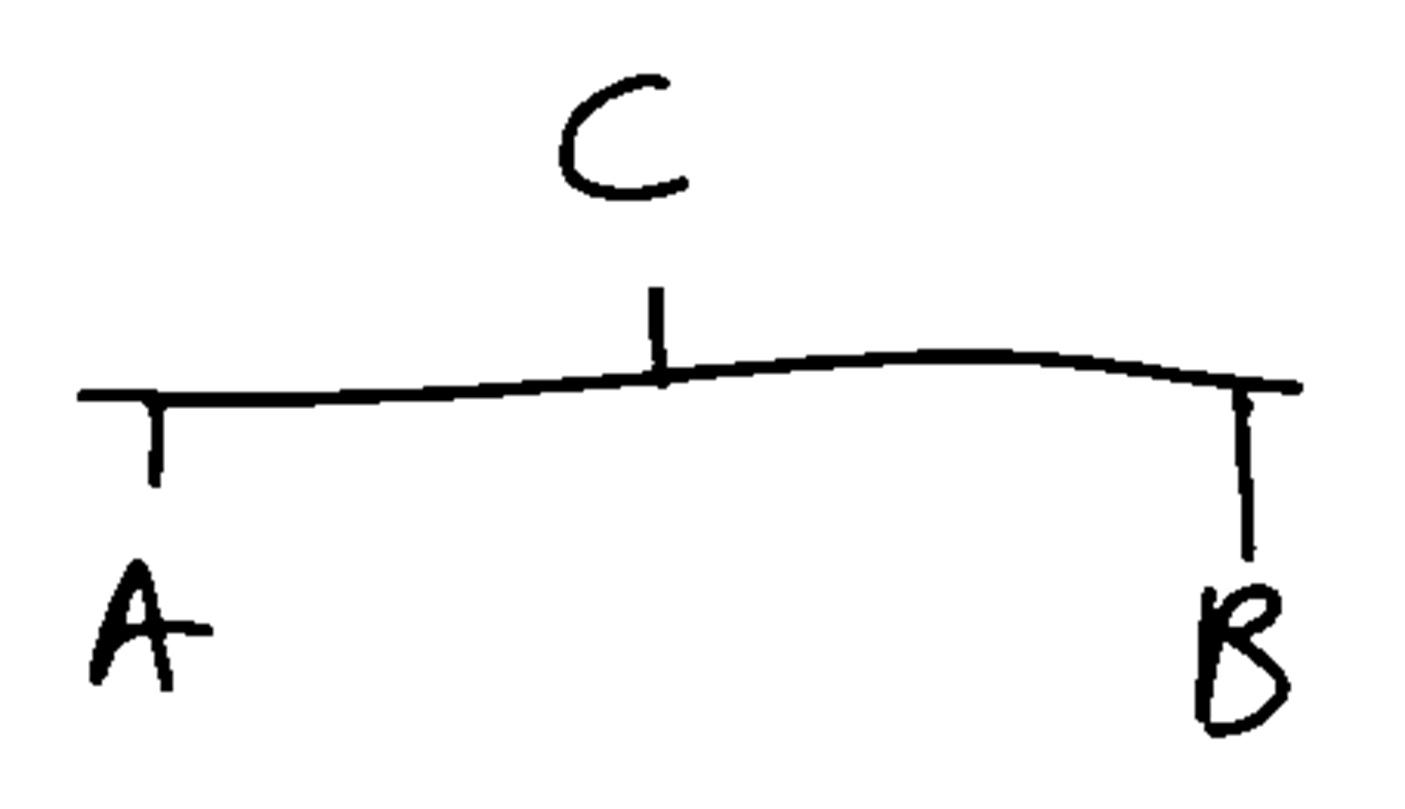
\includegraphics[width=30mm]{cap1 - Introduzione alle reti - 24.jpg}
\end{center}
\noindent Cosa succederebbe se entrambe le stazioni \textit{A} e \textit{B} si mettessero a trasmettere dati alla stazione \textit{C}? Come entrerebbe in gioco il tempo di propagazione in questa situazione?

\noindent Si operava così:
\begin{enumerate}
    \item \textit{Check} disponibilità del cavo: per evitare di interferire quando il cavo non è occupato si aspetta sia libero.
    \item Trasmetto (se libero).
\end{enumerate}
\noindent Ma questo è sufficiente per garantire che il segnale arrivi "pulito" a destinazione?

\noindent No. Può capitare che le due stazioni comincino a trasmettere in contemporanea in assenza di un segnale di "cavo occupato". Più il tempo di trasmissione aumenta, più è facile che il segnale di una stazione incappi in segnali di altre stazioni non visti.
\begin{center}
    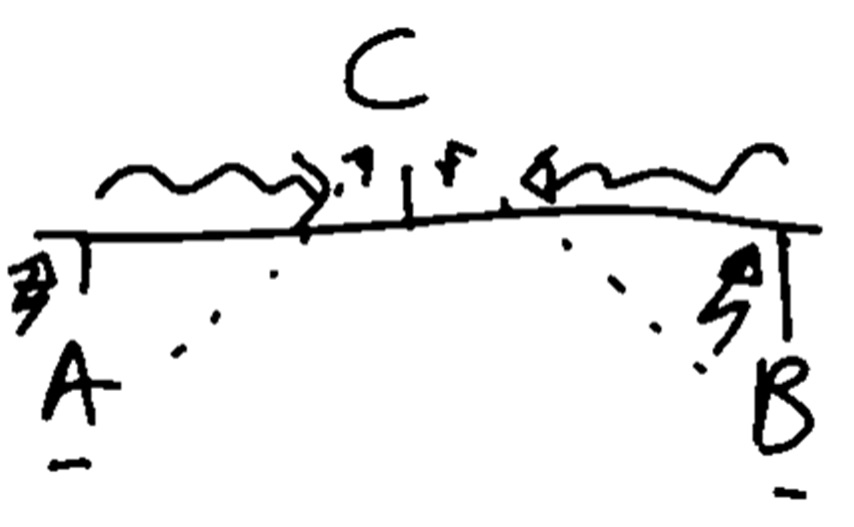
\includegraphics[width=30mm]{cap1 - Introduzione alle reti - 25.jpg}
\end{center}
\noindent La soluzione fu quindi di \textbf{limitare} la lunghezza del cavo. Una lunghezza massima prestabilita di questo cavo semplificava anche i controlli (per assicurarsi che era tutto a posto).

\subsection{Quantificazione del \textit{delay} di trasmissione.}

\noindent È una \textbf{stima} (molto probabilmente lo rivedremo del corso di Ricerca Operativa).
\begin{center}
    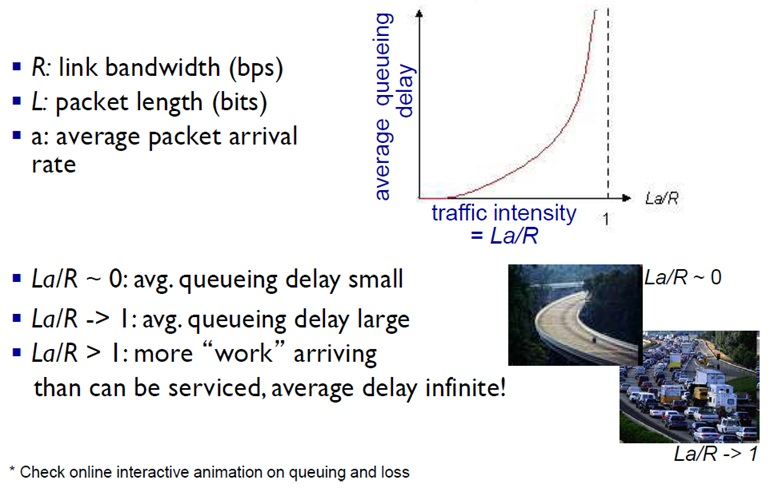
\includegraphics[width=75mm]{cap1 - Introduzione alle reti - 26.jpg}
\end{center}
\noindent In base al valore di $a$ abbiamo più o meno rischi di perdere dati.

\subsection{Simulazione/modellizzazione del \textit{delay} di trasmissione.}

\noindent Questo diagramma riassume un movimento dinamico nel tempo a partire da un utente, attraverso due nodi intermedi (non consideriamo le code) e infine fino ad un server.
\begin{center}
    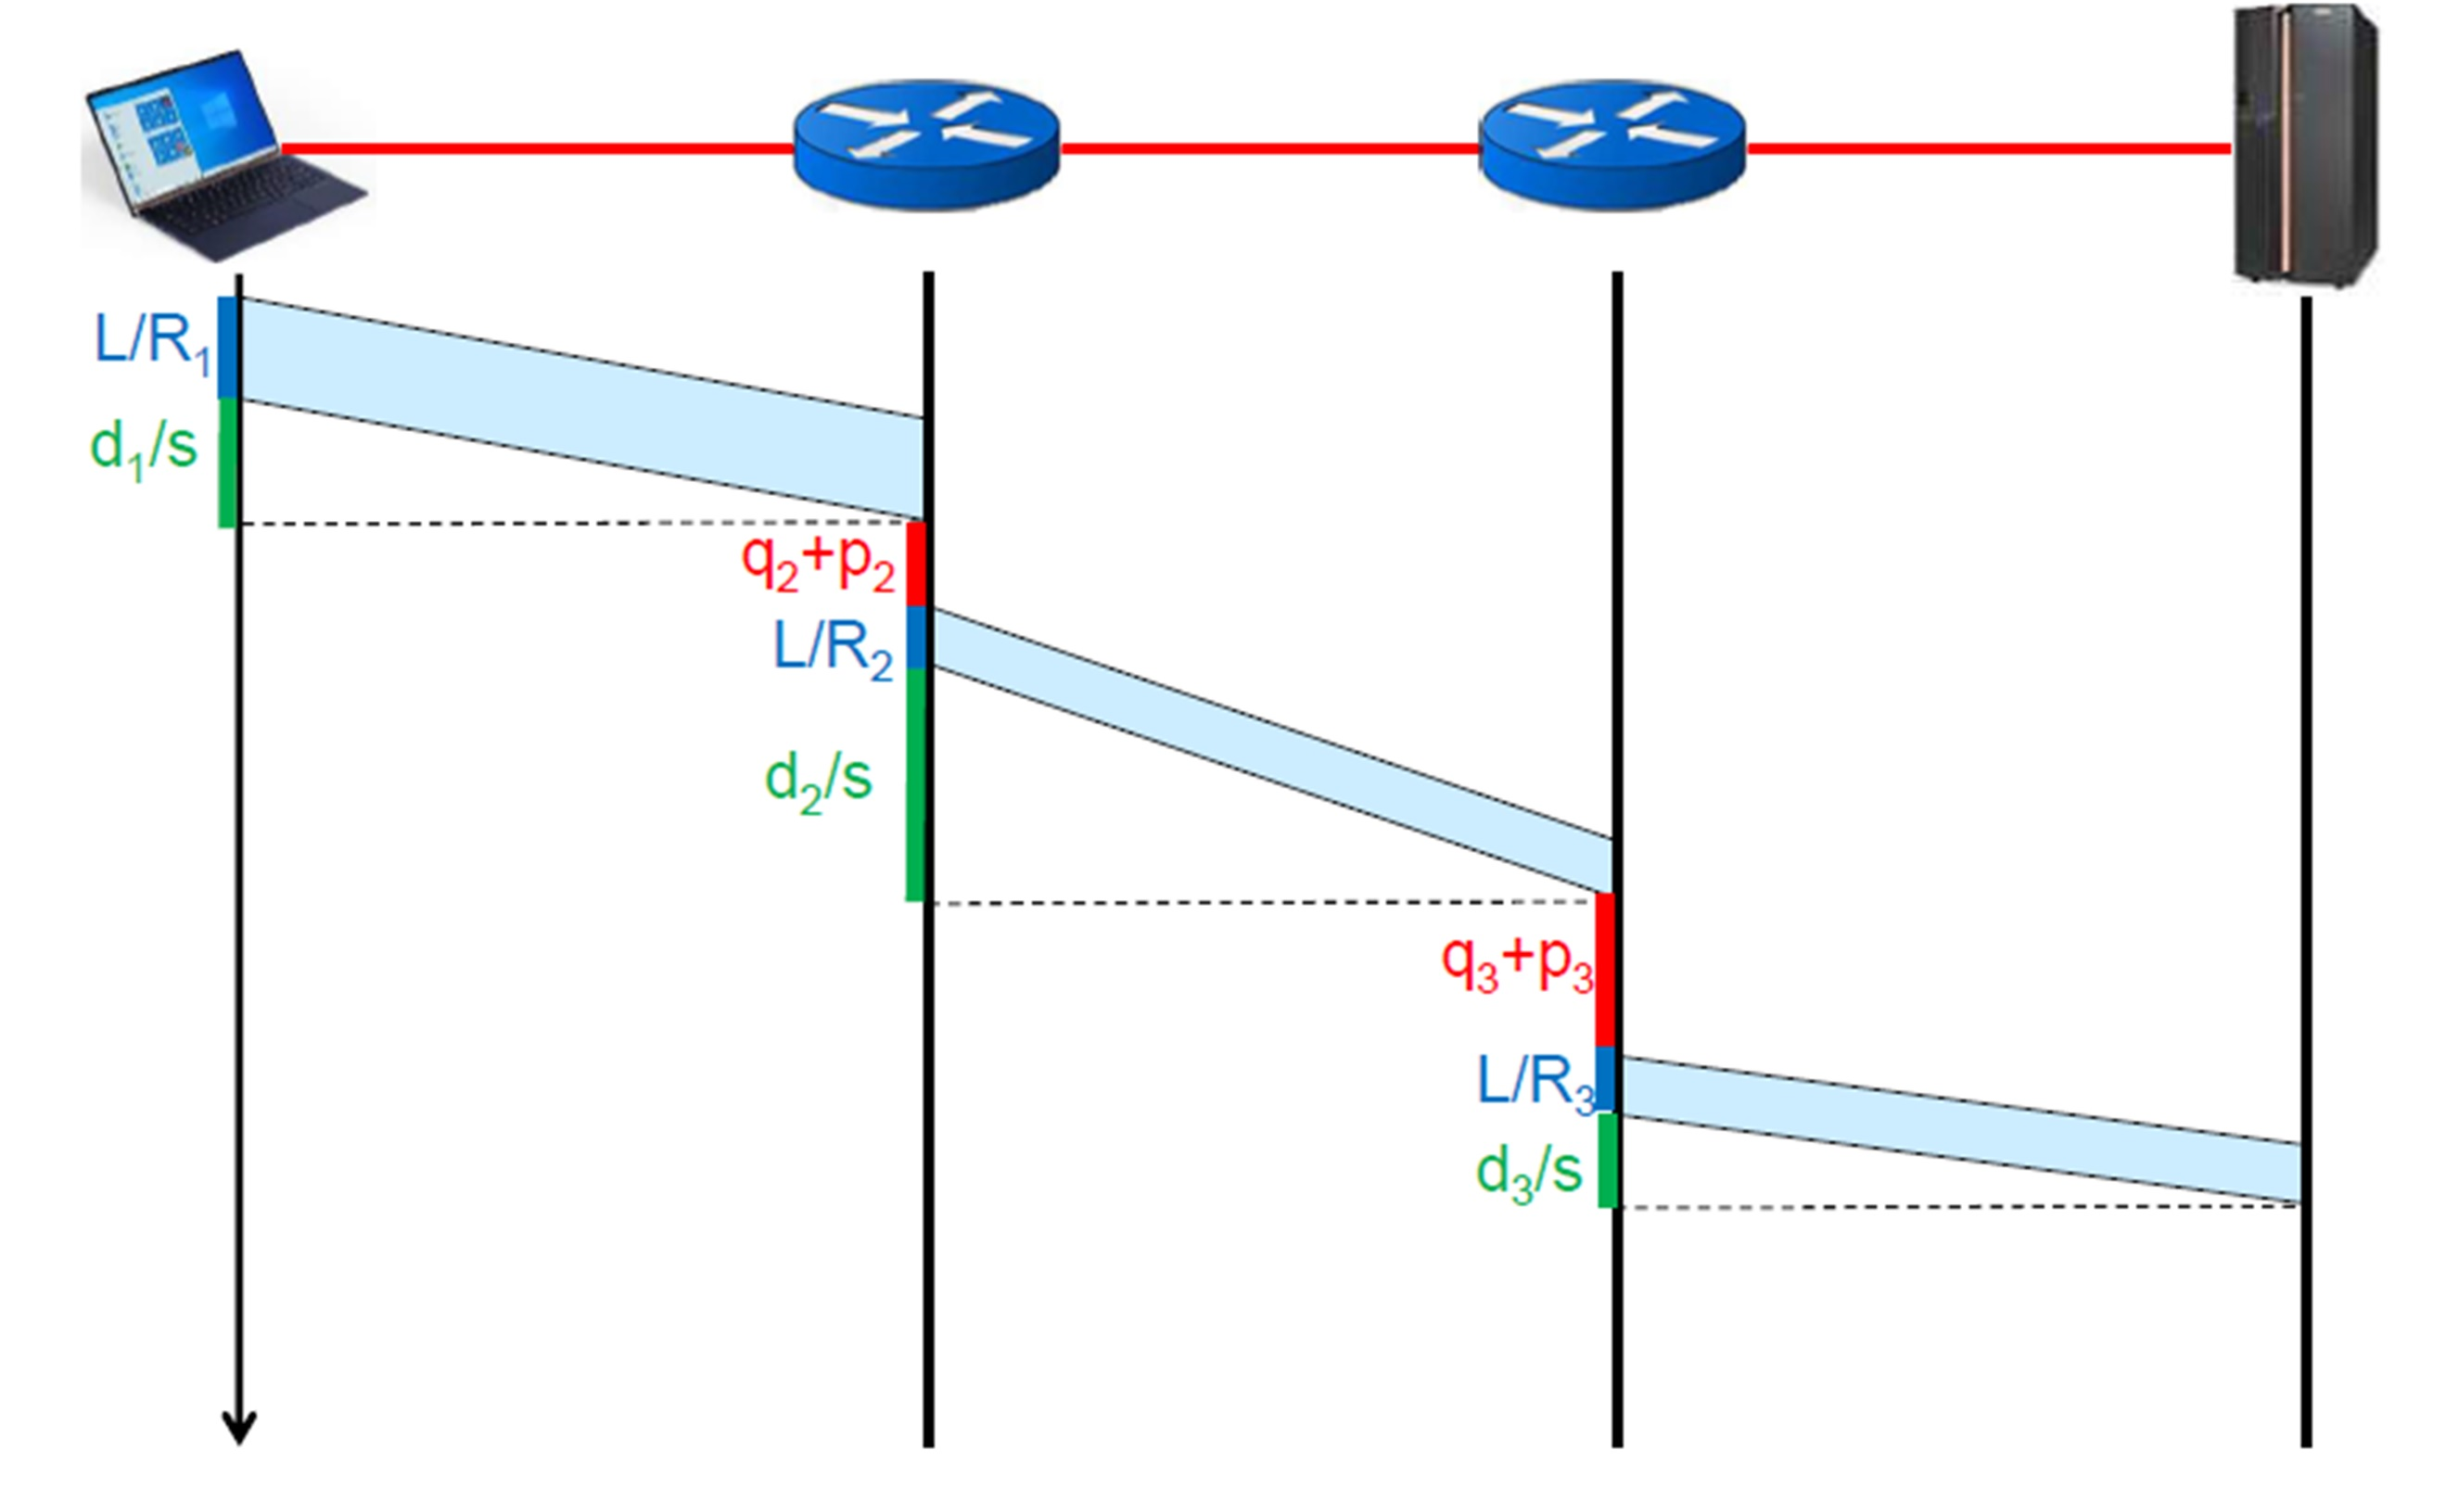
\includegraphics[width=75mm]{cap1 - Introduzione alle reti - 27.jpg}
\end{center}
\noindent Il tempo rappresentato dalla fascia azzurra ($\frac{L}{R}$) è il tempo di \textbf{trasmissione} (numero di $bit$ sulla velocità espressa in $\frac{bit}{sec}$). Qual è il tempo di \textbf{propagazione}? Quello rappresentato in verde, ovvero la distanza fisica del cavo $d$ fratto la velocità di propagazione $s$, $\frac{d}{s}$.

\noindent In rosso sono rappresentati anche il tempo di \textbf{accodamento} (\textit{queue}) e di \textbf{elaborazione} (\textit{processing}).

\noindent N.B.: guardando solo il tempo di propagazione dei due nodi intermedi, si vede in base a quanto alta è la fascia del tempo di propagazione che il primo nodo è più lento del secondo.

\noindent Una situazione più realistica è possibile vederla grazie al comando \textit{\textbf{traceroute}} (provato e commentato nella sezione 1.6.1 dei miei appunti).

\section{La struttura di Internet: rete di reti.}
\begin{center}
    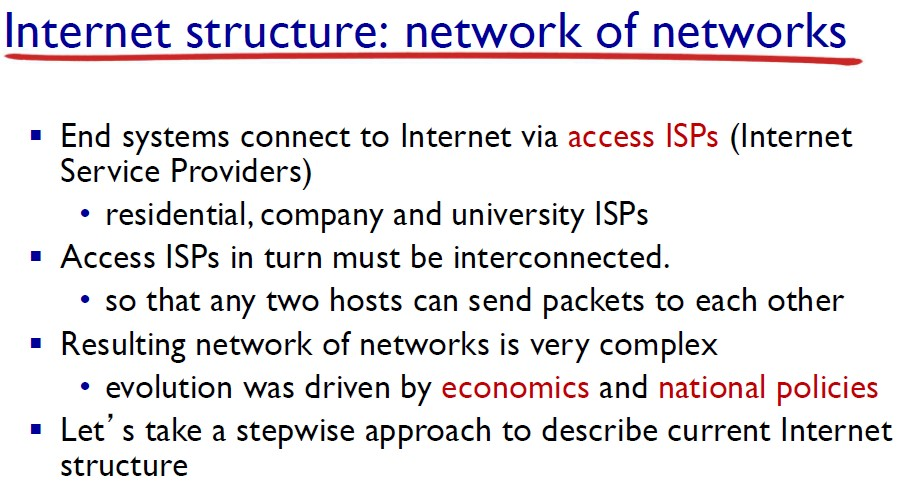
\includegraphics[width=60mm]{cap1 - Introduzione alle reti - 11.jpg}
\end{center}
\begin{center}
    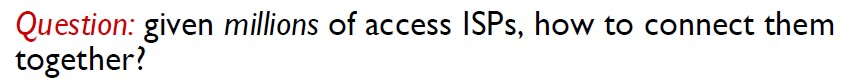
\includegraphics[width=60mm]{cap1 - Introduzione alle reti - 12.jpg}
\end{center}
\begin{center}
    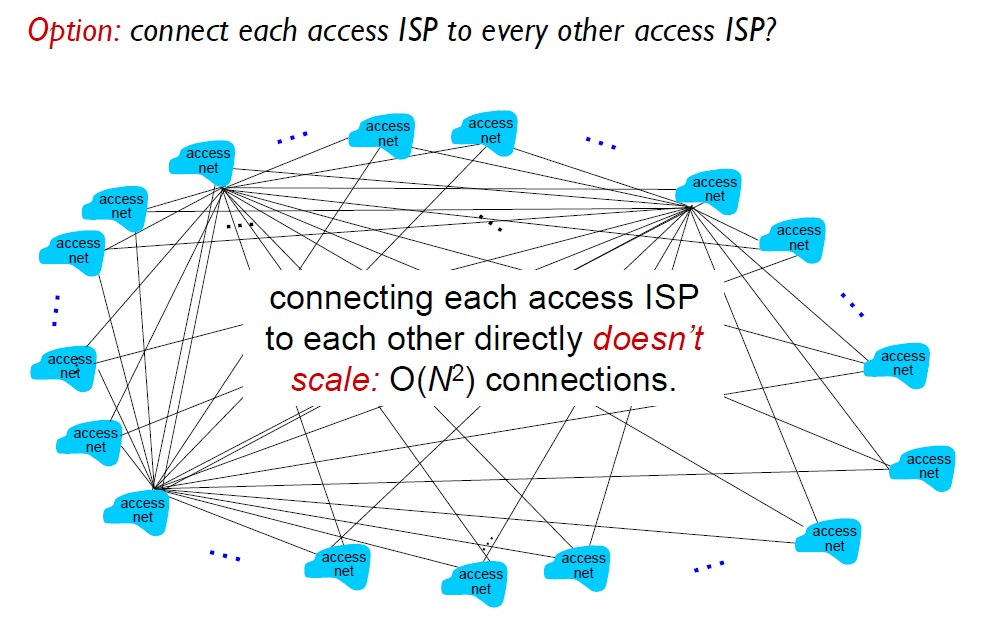
\includegraphics[width=60mm]{cap1 - Introduzione alle reti - 13.jpg}
\end{center}
\noindent Consideriamo per esempio un insieme di utenze (tipo aziende) tutte collegate fra loro. È chiaro che se avessimo $n$ aziende avremmo così un numero di collegamenti spropositato, dell'ordine di grandezza di $O(n^2)$. Poco pratico.
\begin{center}
    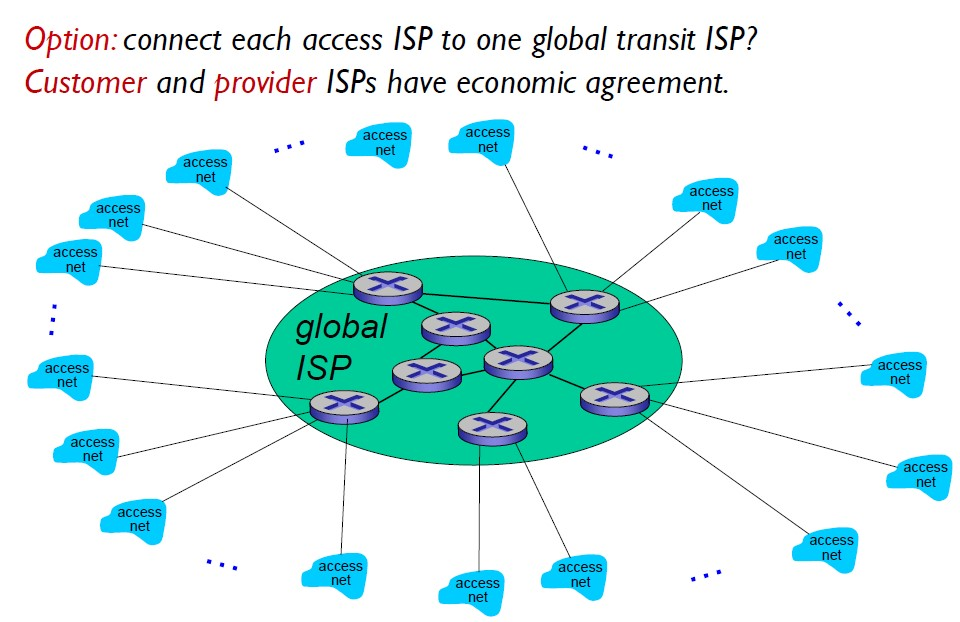
\includegraphics[width=60mm]{cap1 - Introduzione alle reti - 14.jpg}
\end{center}
\noindent Una collaborazione non comporterebbe solo flessibilità ma anche efficienza: con meno collegamenti posso raggiungere più destinatari.
\begin{center}
    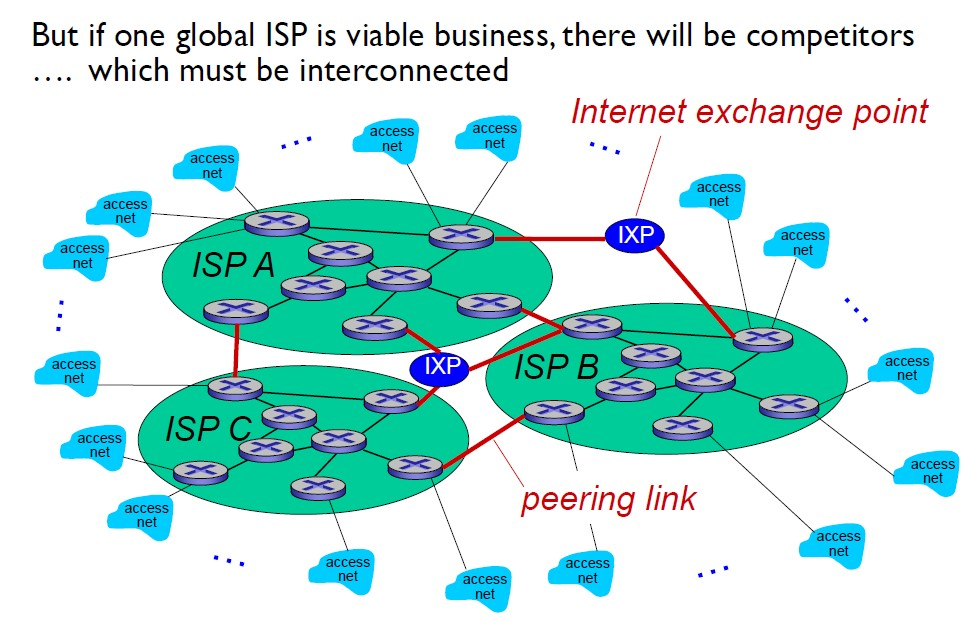
\includegraphics[width=60mm]{cap1 - Introduzione alle reti - 15.jpg}
\end{center}
\noindent Questo porta a particolari accordi fra diversi fornitori (internet providers), ciascuno dotato dei propri clienti che \textit{in proprio} collega fra loro. Semplice. Ma per far comunicare fra loro clienti diversi di providers diversi? Dovranno transitare da altri fornitori.
\begin{center}
    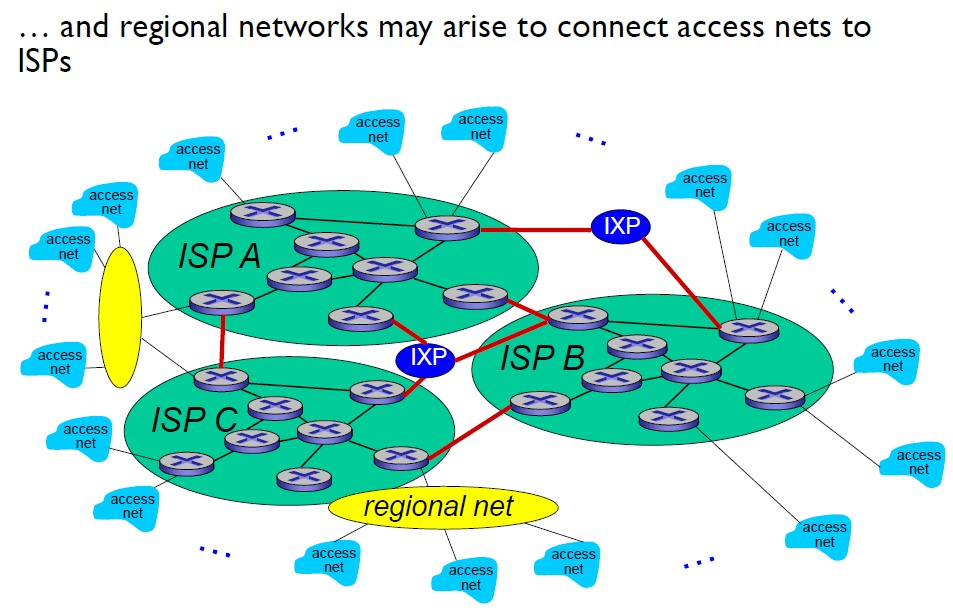
\includegraphics[width=60mm]{cap1 - Introduzione alle reti - 16.jpg}
\end{center}
\noindent Questo è reso possibile in diversi modi:
\begin{itemize}
    \item tramite \textbf{archi diretti}, veri e propri collegamenti fisici.
    \item \textbf{punti di interscambio}, livelli intermedi di collegamento condivisi (e pagati) da più aziende e che danno un punto di scambio per i dati che devono essere trasferiti.
\end{itemize}
\begin{center}
    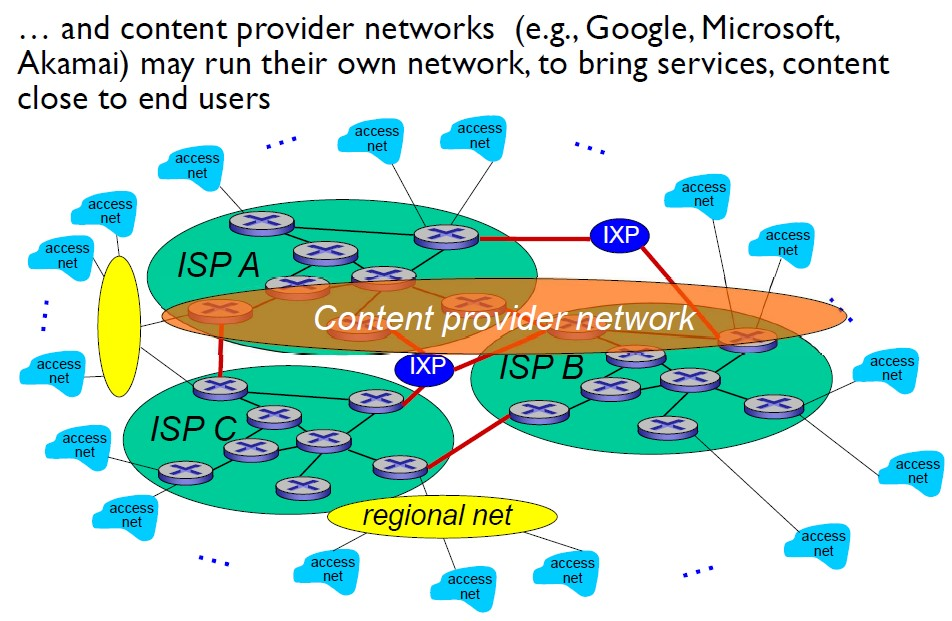
\includegraphics[width=60mm]{cap1 - Introduzione alle reti - 17.jpg}
\end{center}
\noindent Risultato finale:
\begin{center}
    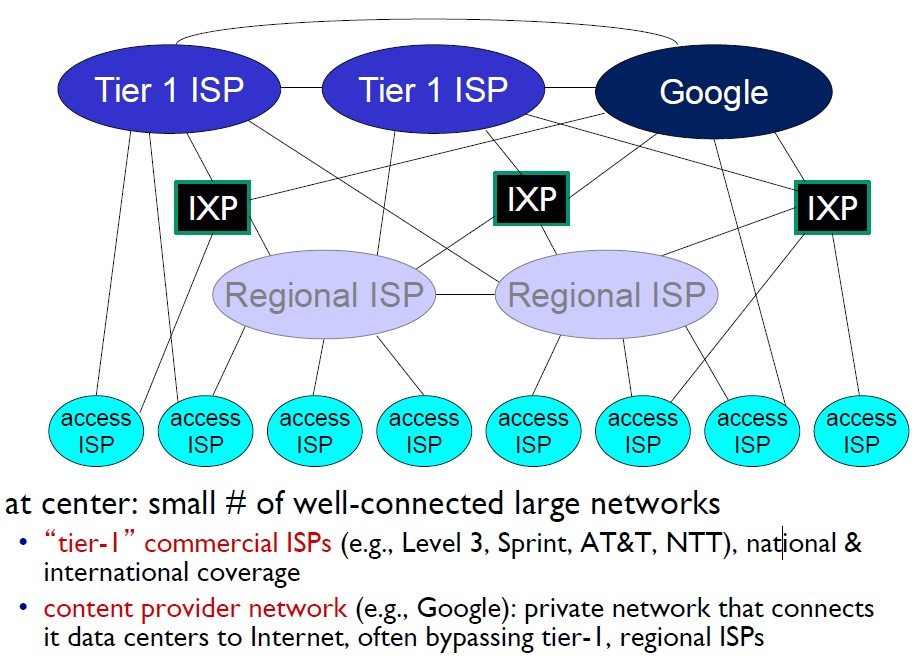
\includegraphics[width=60mm]{cap1 - Introduzione alle reti - 18.jpg}
\end{center}

\section{Prestazioni della rete: throughput.}
\subsection{Throughput: cos'è.}
\noindent Velocità (espressa in $\frac{\text{bit}}{\text{unità di tempo}}$) a cui determinati \textit{bit} in un determinato periodo di tempo vengono trasmessi da mittente a destinatario, ottenuta dopo tutti gli effetti del singolo viaggio.

\noindent Di due tipi:
\begin{itemize}
    \item \textbf{Istantaneo} (\textit{instantaneous t.}): velocità espressa in un punto preciso del percorso.
    \item \textbf{Medio} (\textit{average t.}): velocità espressa in un momento preciso del percorso.
\end{itemize}

\begin{center}
    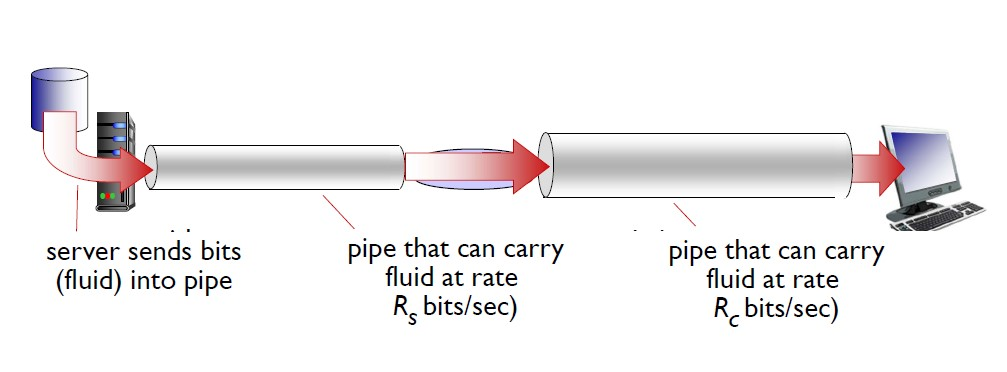
\includegraphics[width=75mm]{cap1 - Introduzione alle reti - 29.jpg}
\end{center}

\subsection{Throughput: visione a "collo di bottiglia".}
\noindent Abbiamo questa situazione: l'informazione passa da una sorgente, attraverso un noto intermedio e fino ad una destinazione. Abbiamo quindi due \textit{throughput} diversi, uno prima ($R_S$) e uno dopo ($R_C$) il nodo intermedio.
\begin{center}
    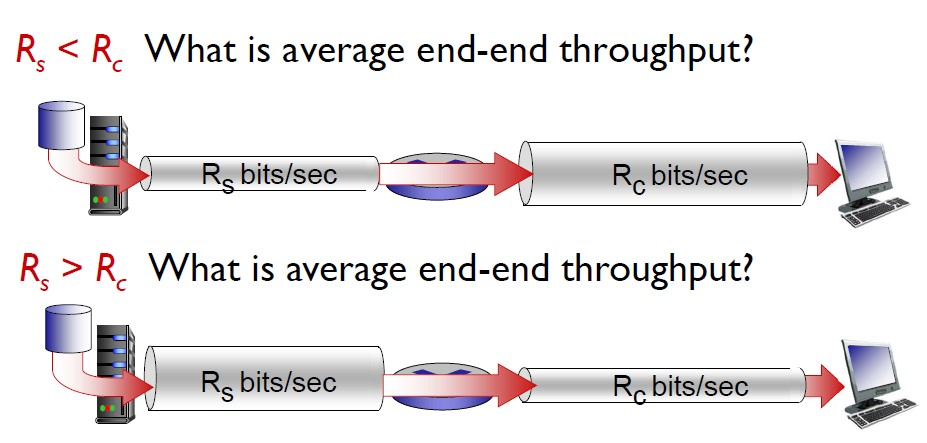
\includegraphics[width=75mm]{cap1 - Introduzione alle reti - 30.jpg}
\end{center}
\noindent Ovviamente la prestazione complessiva dipende dal rapporto che intercorre fra le due $R$.

\noindent È possibile notare che:
\begin{itemize}
    \item se $R_S < R_C$, non ci sarà molta coda di attesa a livello di nodo intermedio essendoci a valle una velocità ($R_C$) consistente;
    \item se $R_S > R_C$, siamo nella situazione opposta ovvero tende a crearsi una coda di attesa decisamente consistente a livello di nodo (con conseguente rischio di \textit{loss} di informazione).
\end{itemize}
\noindent A questa situazione facciamo riferimento quando parliamo di \textit{\textbf{bottleneck link}}, ovvero \textit{collegamento a collo di bottiglia}, che è il tipo di condivisione appena descritta.
\begin{center}
    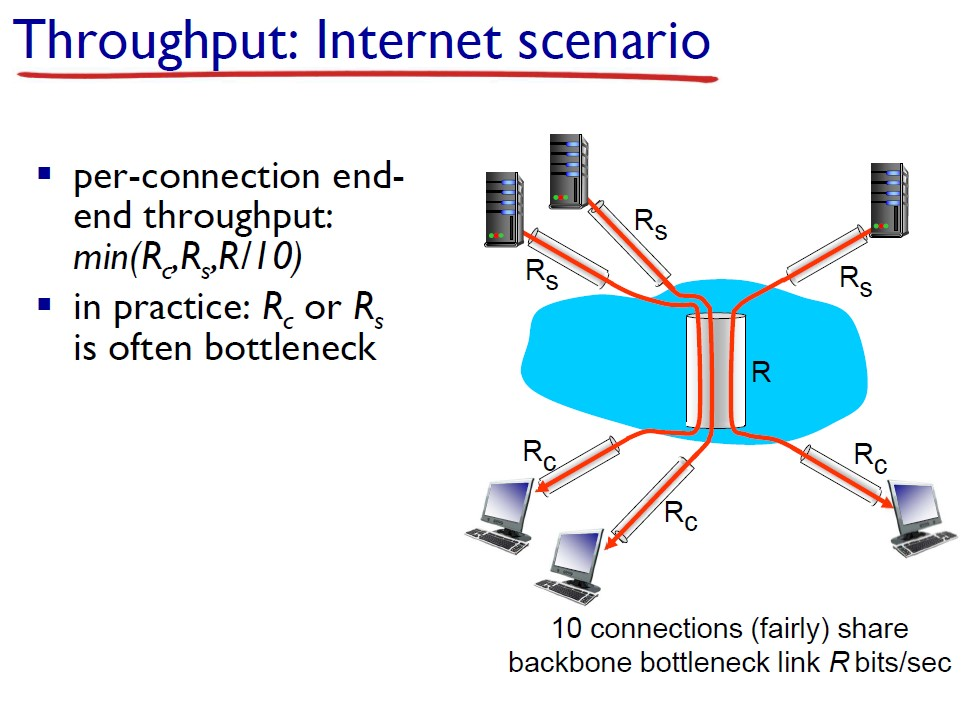
\includegraphics[width=75mm]{cap1 - Introduzione alle reti - 31.jpg}
\end{center}
\noindent N.B.: questa situazione illustra una condivisione (la rete internet) che è \textbf{equa}, parliamo di \textit{neutralità della rete}.

\section{I protocolli di Internet: in breve.}
\noindent Protocolli organizzati in \textit{layers}, che messi assieme costituiscono la nostra rete (concetto base importantissimo).
\subsection{Protocolli e layers.}
\noindent La rete è complessa, composta da molti pezzi (alcuni anche materiali) che collaborano fra loro.
\begin{itemize}
    \item \underline{\textbf{hosts}}: sono le macchine di terminale (\textit{edge});
    \item \underline{\textbf{routers}}: sono le macchine interne che instradano;
    \item \underline{\textbf{links of various media}}: sono collegamenti con vari supporti fisici (\textit{media}) quindi cavo, fibra...
    \item \underline{\textbf{applications}}: sono elementi software che fanno generazione del traffico (applicazioni, browser, server web...);
    \item \underline{\textbf{protocols}}: sono standard che mettono in collaborazione correttamente i vari elementi;
    \item \underline{\textbf{hardware, software}}: vario supporto hardware, schede...
\end{itemize}
\noindent Tutti questi elementi hanno esigenze diverse ma devono collaborare per un buon funzionamento complessivo. 

\noindent Come è possibile fare ciò? Organizzandoli per \textit{\textbf{ambiti}} o \textit{\textbf{livelli}}.

\noindent Questa divisione deve essere standardizzata, cioè serve avere un accordo sulla terminologia e le definizioni. Questa \textit{compartimentazione}, questa \textit{modularità}, semplifica ogni valutazione o aggiornamento senza doversi coordinare con il \textit{resto} del sistema (solo con una o due parti, ovvero quelle immediatamente adiacenti a quella dove mi trovo).

\subsection{Internet come una cooperazione.}
\noindent Tutto quello di cui abbiamo parlato finora dipende da una cooperazione fra \textbf{tecnologie} e \textbf{standard} (non prodotti, i prodotti implementano gli standard, es. Chrome implementa HTTP), gli ultimi sono divisi per \textbf{funzionalità}. I vari standard collaborano fra loro secondo una struttura verticale, basandosi sulla \textit{adiacenza} o \textit{contiguità}: un livello può quindi comunicare esclusivamente con il livello immediatamente precedente o immediatamente successivo.
\begin{center}
    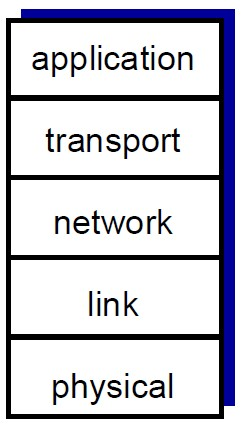
\includegraphics[width=15mm]{cap1 - Introduzione alle reti - 19.jpg}
\end{center}
\begin{itemize}
    \item \textbf{\underline{Livello applicativo}: supporta applicazioni di rete.} Es.: HTTP.
    
    Sono tutto il nostro software utente. Non le vedremo in dettaglio, ci interessa sapere che l'applicazione che vuole scambiare dati con un server web deve farlo rispettando un protocollo (HTTP).

    \textit{Client $+$ server}: sono a livello applicativo entrambi implementazioni di HTTP.
    \item \textbf{\underline{Livello di trasporto}: trasferisce dati fra processi.} Es.: TCP, UDP.

    Il livello trasporto si occupa di "far vedere la rete all'applicazione". Quest'ultima se ne frega dei pacchetti dei dati. Il trasporto non fa vedere il pacchetto ma internamente è obbligato a frazionare i dati da trasferire in pacchetti. Perciò il compito del livello di trasposto è di collaborare con i livelli immediatamente adiacenti, uno sta sopra l'altro sta sotto.
    
    Due esempi di protocollo (quelli citati) sono TCP, dove c'è garanzia di consegna, e UDP, che invece butta in giro pacchetti dimenticandosene (non completamente inutile, per condivisioni di dati come per esempio multimediali va benissimo UDP).
    \item \textbf{\underline{Livello di rete}: routing di dati (mittente$\rightarrow$destinatario).} Es.: IP.
    
    Il livello di rete mette in collaborazione i nodi fra loro; quando c'è collaborazione, è il livello di rete a decidere l'instradamento. Non solo, si occupa anche di identificare mittente e destinatario.

    Perciò  \textit{livello di rete $=$ identificazione $+$ instradamento}.
    \item \textbf{\underline{Livello di data link}: trasferimento di dati tra elementi di rete adiacenti.} Es.: Ethernet.
    
    Gestisce il trasferimento di dati fra nodi adiacenti. Il livello di data link si concentra sul singolo arco e ignora cosa gli sta intorno, organizza il salto dei dati mettendosi d'accordo con chi "sta sopra" e chi "sta sotto": sotto dettatura dell'instradamento, fa un singolo salto sapendo già su quale livello fisico deve andare.
    \item \textbf{\underline{Livello fisico}: i bit sul cavo fisico.}

    Un altro livello presentato superficialmente. Ne abbiamo parlato in dettaglio nelle sezioni 1.3-1.6.

    Il livello fisico ha rilevanza per quanto riguarda la sicurezza: è chiaro che un livello fisico via segnale radio sarà più fragile parlando di sicurezza rispetto ad un collegamento via cavo (ci sono corsi universitari appositi, ma per fare un esempio è per questo che quando si parla di connessioni wireless si vede anche la loro crittografia, perché sono connessioni poco sicure).
\end{itemize}

\subsection{Esempio pratico di trasferimento di un dato.}
\noindent Quest'immagine rappresenta l'output di un comando che cerca di farmi vedere cosa accade quando cerco di mandare un dato a destinazione. Il comando è \textit{traceroute (tracert)}. Come funziona? Chiede la destinazione che si vuole raggiungere e fa vedere ogni salto intermedio di comunicazione.
\begin{center}
    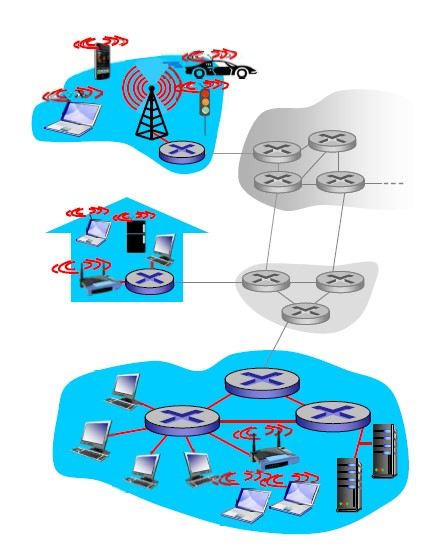
\includegraphics[width=40mm,scale=0.5]{cap1 - Introduzione alle reti - 2.jpg}
\end{center}
\noindent Nell'esempio raffigurato, presumibilmente si è cercato di far partire il dato dalla sede degli autori del libro ("umass") verso una macchina per loro dall'altra parte dell'oceano (in Francia, ".fr"). I salti compiuti sono almeno 19 (infatti abbiamo 19 righe): abbiamo un mittente, un destinatario e 17 nodi intermedi. È possibile vedere ad ogni step l'\textit{identità tecnica} (IP) delle macchine attraversate e l'\textit{identità più umana} (lo vedremo col sistema \textit{vbns}). Poi vengono fatti esperimenti di comunicazione (tre volte per ogni nodo intermedio) e vengono registrati i tempi per ognuno dei messaggi inviati.

\noindent Nell'esempio raffigurato, è possibile notare un considerevole aumento del tempo di transito (\textit{delay}) che potrebbe corrispondere al salto al di là dell'oceano.

\noindent Ma perché \underline{\textit{tre}} misurazioni? Perché noi sappiamo che la rete \textit{fa del suo meglio} (best-effort); per avere un'indicazione approssimativa ma affidabile si fanno tre misurazioni, anche per evitare situazioni transitorie e non ottimali che potrebbero dare una misurazione non accurata.
\begin{center}
    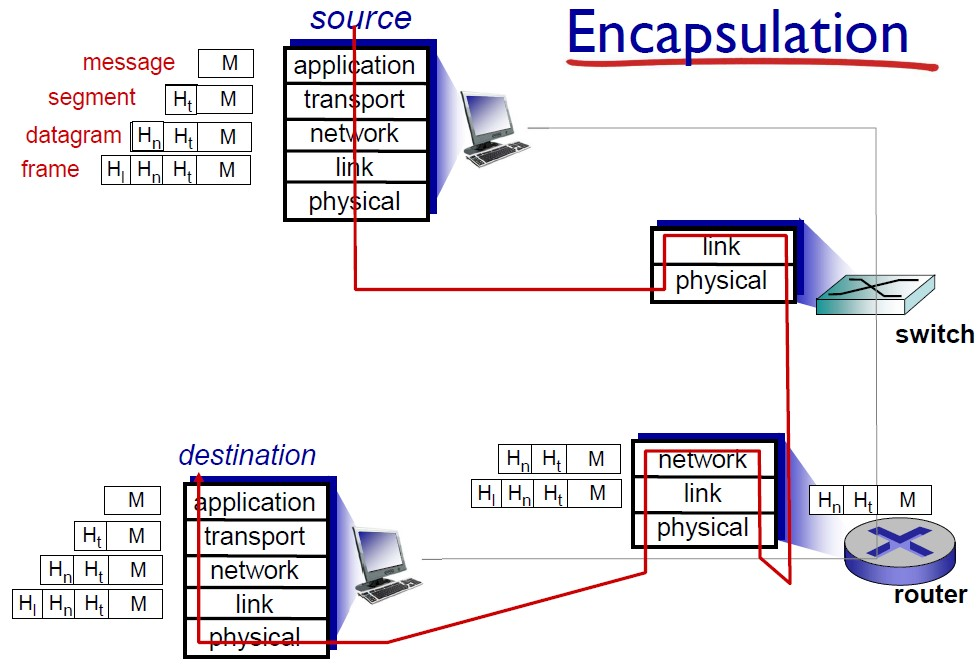
\includegraphics[width=80mm,scale=0.5]{cap1 - Introduzione alle reti - 32.jpg}
\end{center}

\chapter{Strato di trasporto}
Capitolo 3 (Kurose-Ross 7a edizione).

\noindent Paragrafi: 3.1 - 3.7 (escluso 3.4.1, "Building a Reliable Data Transfer Protocol", 3.5.2, "TCP Segment Structure", 3.5.3 "Round-Trip Time Estimation and Timeout")

\section{Servizi e protocolli del livello di Trasporto.}
\noindent Questo livello si occupa di fornire \textbf{comunicazione logica} tra i processi di applicazioni in esecuzione su \textit{hosts} diversi.

\noindent Cosa succede nel \textit{lato mittente}: si occupa di spezzare i messaggi delle applicazioni in \textbf{\textit{segmenti}} che passa poi al livello di rete.

\noindent Cosa succede nel \textit{lato destinatario}: si occupa di riassemblare i segmenti in messaggi che manda poi al livello applicativo.
\begin{center}
    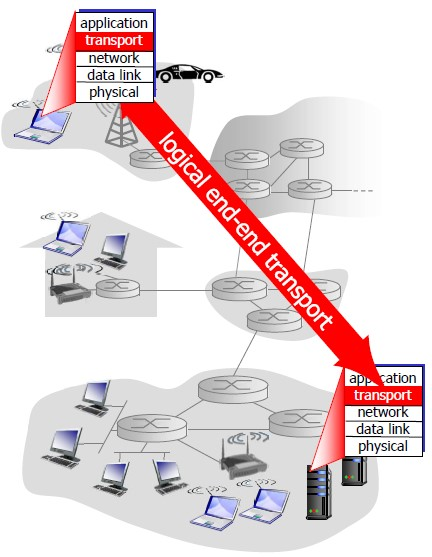
\includegraphics[width=50mm]{cap2 - Livello di Trasporto - 1.jpg}
\end{center}
\noindent C'è più di un tipo di protocollo per il livello di trasporto, Internet per esempio usa sia \textbf{TCP} che \textbf{UDP}.

\subsection{Livello di trasporto vs Livello di rete.}
\noindent Il livello di \textit{rete} si occupa della comunicazione logica fra \textit{hosts} (saltando di nodo in nodo).

\noindent Il livello di \textit{trasporto} si occupa della comunicazione logica fra \textit{processi} (si appoggia sul livello di rete per mandare i singoli pezzetti).

\noindent Il bello del lavorare su più \textit{layers} è proprio l'indipendenza delle singole operazioni (cioè "ognuno si fa gli affari suoi") che però collaborano per supportare ciò che sta sopra. Per esempio: il livello di trasporto ha sopra quello di applicazione e deve lavorare per distinguere fra le varie applicazioni che ci sono sulla macchina chi è quella coinvolta, il livello di rete che sta sopra al livello di trasporto non si deve preoccupare di tutto ciò, ma solo di rapportarsi col livello di trasporto per prendere il pezzo di dato con cui fare il suo lavoro.

\subsection{I protocolli Internet del livello di trasporto.}
\noindent Abbiamo parlato dei protocolli Internet per il livello di trasporto, \textbf{TCP} e \textbf{UDP}.

\noindent Principali differenze:
\begin{itemize}
    \item \textbf{\textit{TCP}}: è affidabile, garantisce (finché può) la consegna dei dati. Si occupa di:
    \begin{itemize}
        \item controllo del flusso (eventuali attese, dimensioni dei pacchetti, etc.);
    \end{itemize}
    \item \textbf{\textit{UTP}}: è
\end{itemize}
% 11:45


























\chapter{Strato di rete}
\section{Rappresentazione dell'informazione}
\begin{itemize}
    \item Sistemi numerici
    \item Rappresentazione dei numeri interi con e senza segno
    \item Rappresentazione dei numeri in virgola fissa e mobile
    \item Rappresentazione dell'informatica non numerica
\end{itemize}

\chapter{Introduzione ai sistemi operativi}
\section{Rappresentazione dell'informazione}
\begin{itemize}
    \item Sistemi numerici
    \item Rappresentazione dei numeri interi con e senza segno
    \item Rappresentazione dei numeri in virgola fissa e mobile
    \item Rappresentazione dell'informatica non numerica
\end{itemize}

\chapter{Processi e thread}
\section{Rappresentazione dell'informazione}
\begin{itemize}
    \item Sistemi numerici
    \item Rappresentazione dei numeri interi con e senza segno
    \item Rappresentazione dei numeri in virgola fissa e mobile
    \item Rappresentazione dell'informatica non numerica
\end{itemize}

\chapter{Scheduling della CPU}
\section{Rappresentazione dell'informazione}
\begin{itemize}
    \item Sistemi numerici
    \item Rappresentazione dei numeri interi con e senza segno
    \item Rappresentazione dei numeri in virgola fissa e mobile
    \item Rappresentazione dell'informatica non numerica
\end{itemize}

\chapter{Livello di data link e LAN}
\section{Rappresentazione dell'informazione}
\begin{itemize}
    \item Sistemi numerici
    \item Rappresentazione dei numeri interi con e senza segno
    \item Rappresentazione dei numeri in virgola fissa e mobile
    \item Rappresentazione dell'informatica non numerica
\end{itemize}

\chapter{Reti wireless}
\section{Rappresentazione dell'informazione}
\begin{itemize}
    \item Sistemi numerici
    \item Rappresentazione dei numeri interi con e senza segno
    \item Rappresentazione dei numeri in virgola fissa e mobile
    \item Rappresentazione dell'informatica non numerica
\end{itemize}

\chapter{Gestione della memoria}
\section{Rappresentazione dell'informazione}
\begin{itemize}
    \item Sistemi numerici
    \item Rappresentazione dei numeri interi con e senza segno
    \item Rappresentazione dei numeri in virgola fissa e mobile
    \item Rappresentazione dell'informatica non numerica
\end{itemize}

\chapter{File system}
\section{Rappresentazione dell'informazione}
\begin{itemize}
    \item Sistemi numerici
    \item Rappresentazione dei numeri interi con e senza segno
    \item Rappresentazione dei numeri in virgola fissa e mobile
    \item Rappresentazione dell'informatica non numerica
\end{itemize}

\chapter{Macchine virtuali}
\section{Rappresentazione dell'informazione}
\begin{itemize}
    \item Sistemi numerici
    \item Rappresentazione dei numeri interi con e senza segno
    \item Rappresentazione dei numeri in virgola fissa e mobile
    \item Rappresentazione dell'informatica non numerica
\end{itemize}

\end{document}